\documentclass{article}
\usepackage{hyperref}
\usepackage{comment}
\usepackage{longtable}
\usepackage{array}
\usepackage{graphicx}
\usepackage{fancyhdr}
\usepackage[italian]{babel}
\usepackage{amsmath}
\usepackage{enumitem}
%\usepackage{geometry}

\usepackage{tikz} %copertina
\usetikzlibrary{shapes.geometric, calc} %copertina
\usepackage{xcolor} %copertina

\usepackage{listings} %sql
\lstset{
    language=SQL, 
    basicstyle=\small\ttfamily,
    numbers=left, 
    numberstyle=\tiny, 
    frame=line,
    keywordstyle=\color{blue},
    commentstyle=\color{red},
    stringstyle=\color{orange},
    identifierstyle=\color{black},
    numberstyle=\tiny\color{black},
    breaklines=true,
    linewidth=1.185\linewidth
}

\hypersetup{
    colorlinks=true,
    linkcolor=black,      % Colore del testo del link
    citecolor=blue,      % Colore delle citazioni nel testo
    urlcolor=blue,       % Colore degli URL
    linkbordercolor=blue, % Colore del bordo del link
    citebordercolor=blue, % Colore del bordo delle citazioni nel testo
    urlbordercolor=blue,  % Colore del bordo degli URL
    pdfborderstyle={/S/U/W 1}, % Stile del bordo del link (sottolineato)
}

\begin{document}

\begin{tikzpicture}[overlay,remember picture]

\definecolor{Dandelion}{RGB}{240, 225, 48} % Esempio di definizione del colore Dandelion
\definecolor{orange}{RGB}{255, 165, 0} % Esempio di definizione del colore orange
\definecolor{RoyalBlue}{RGB}{65, 105, 225} % Esempio di definizione del colore RoyalBlue
\definecolor{Emerald}{RGB}{46, 204, 113} % Definizione del colore Emerald
\definecolor{OrangeRed}{RGB}{255, 69, 0} % Definizione del colore OrangeRed

\global\def\THETITLE{\selectfont \bf Documetazione Data Base}
\global\def\SUBTITLE{Sistema di gestione di una pagina wiki}
\global\def\THEAUTHOR{Raffaele Raia e Florindo Zecconi}% set document author
\global\def\THEUNIVERSITY{Università di Napoli Federico 	II}% set document university

	% Background color
	%\fill[black!2](current page.south west) rectangle (current page.north east);
	\fill[white!2](current page.south west) rectangle (current page.north east);
	
%	\node[opacity=0.1,left color=white] (image) at (-2,-20) {\includegraphics[scale=1.5, angle=-15,origin=c]{logo-simple}};
		
	\node[opacity=0.1,left color=white] (image) at ($(current page.south east)+(-3.3, 2.0)$) {
\includegraphics[scale=2.25, angle=4,origin=c]{Copertina/F2logobianco.jpg}};
	
	% Rectangles
	\shade[left color=Dandelion, right color=blue!40, transform canvas ={rotate around ={45:($(current page.north west)+(0,-6)$)}}] ($(current page.north west)+(0,-6)$) rectangle ++(9,1.5);
	
	\shade[left color=lightgray,right color=blue!50, rounded corners=0.75cm,transform canvas ={rotate around ={45:($(current page.north west)+(0.9,-9.5)$)}}]($(current page.north west)+(0.9,-9.5)$) rectangle ++(15,1.5);
	
%	\shade[left color=lightgray, rounded corners=0.3cm, transform canvas ={rotate around ={45:($(current page.north west)+(.5,-10)$)}}] ($(current page.north west)+(1.5,-9.55)$) rectangle ++(7,.6);
	
	\shade[left color=orange!80, right color=blue!60, rounded corners=0.4cm, transform canvas ={rotate around ={45:($(current page.north)+(-1.5,-3)$)}}] ($(current page.north)+(-1.5,-3)$) rectangle ++(9,0.8);
	
	\shade[left color=red!80, right color=blue!80, rounded corners=0.9cm, transform canvas ={rotate around ={45:($(current page.north)+(-3,-8)$)}}] ($(current page.north)+(-3,-8)$) rectangle ++(15,1.8);
	
	\shade[left color=orange, right color=blue, rounded corners=0.9cm, transform canvas ={rotate around ={45:($(current page.north west)+(4,-15.5)$)}}]
	($(current page.north west)+(4,-15.5)$) rectangle ++(30,1.8);
	
	\shade[left color=RoyalBlue, right color=Emerald, rounded corners=0.75cm, transform canvas ={rotate around ={45:($(current page.north west)+(13,-10)$)}}] ($(current page.north west)+(13,-10)$) rectangle ++(15,1.5);
	
	\shade[left color=OrangeRed, right color=RoyalBlue!80, rounded corners=0.3cm, transform canvas ={rotate around ={45:($(current page.north west)+(18,-8)$)}}] ($(current page.north west)+(18,-8)$) rectangle ++(15,0.6);
	
	\shade[left color=OrangeRed, right color=RoyalBlue!80, rounded corners=0.4cm, transform canvas ={rotate around ={45:($(current page.north west)+(19,-5.65)$)}}] ($(current page.north west)+(19,-5.65)$) rectangle ++(15,0.8);
	
	\shade[left color=OrangeRed, right color=RoyalBlue!80, rounded corners=0.6cm, transform canvas ={rotate around ={45:($(current page.north west)+(20,-9)$)}}] ($(current page.north west)+(20,-9)$) rectangle ++(14,1.2);
	
	% Year
%	\draw[ultra thick,gray]($(current page.center)+(5,2)$) -- ++(0,-3cm) 
%	node[midway, left=0.25cm, text width=10cm, align=right, black!75] {
%		
%		{\fontsize{25}{30} \selectfont \bf Sistema di gestione di una pagina wiki \\[10pt]}
%	}
%	node[midway, right=0.25cm, text width=6cm, align=left, orange] {
%
%		{\fontsize{72}{86.4} \selectfont \coverdate\today}
%	};
	
	% Title
	\node[align=center] at ($(current page.center)+(0,-5)$) {
		{
\includegraphics[scale=0.1]{Copertina/pixlr-image-generator-b77a4501-372c-489b-8045-1161501d516d-PhotoRoom.png-PhotoRoom.png}}\\[1cm]
  
		{\fontsize{40}{72} \selectfont {\THETITLE}} \\[1cm]
        {\fontsize{35}{72} \selectfont {\SUBTITLE}} \\[1cm]
		{\fontsize{16}{19.2} \selectfont \textcolor{orange}{ \bf \THEAUTHOR}}\\[3pt]
		\THEUNIVERSITY\\[3pt]
        \today
	};

\end{tikzpicture}

\newpage

\tableofcontents

\newpage

\pagestyle{fancy}
\fancyhead[L]{ }

\section{Progettazione Concettuale}

\subsection{Analisi dei Requisiti}



\subsubsection{Traccia}
%\begin{comment}
\textit{“Una pagina di una wiki ha un titolo e un testo. Ogni pagina è creata da un determinato autore. Il
testo è composto di una sequenza di frasi. Il sistema mantiene traccia anche del giorno e ora nel quale la pagina è stata creata. La pagina può contenere anche dei collegamenti. Ogni collegamento è caratterizzato da una frase da cui scaturisce il collegamento e da un’altra pagina destinazione del collegamento.}\newline

\textit{Il testo può essere modificato da un altro utente del sistema, che seleziona una o più delle frasi, scrive la sua versione alternativa (modifica) e prova a proporla.}\newline

\textit{La modifica proposta verrà notificata all’autore del testo originale la prossima volta che utilizzerà il sistema.}\newline

\textit{L’autore potrà vedere la sua versione originale e la modifica proposta. Egli potrà accettare la modifica (in quel caso la pagina originale diventerà ora quella con la modifica apportata), rifiutare la modifica (la pagina originale rimarrà invariata). La modifica proposta dall’autore verrà memorizzata nel sistema e diventerà subito parte della versione corrente del testo. Il sistema mantiene memoria delle modifiche proposte e anche delle decisioni dell’autore (accettazione o rifiuto).}\newline

\textit{Nel caso in cui si fossero accumulate più modifiche da rivedere, l’autore dovrà accettarle o rifiutarle tutte nell’ordine dalla più antica alla più recente."}

\textit{Gli utenti generici del sistema potranno cercare una pagina e il sistema mostrerà la versione corrente del
testo e i collegamenti.
Gli autori dovranno prima autenticarsi fornendo la propria login e password. Tutti gli autori potranno vedere
tutta la storia di tutti i testi dei quali sono autori e di tutti quelli nei quali hanno proposto una modifica.}

%\end{comment}
\subsubsection{Preambolo}
La prima fase della progettazione consiste nell'analisi dei requisiti. Qui verranno identificate le informazioni principali che porteranno allo sviluppo della struttura del data base per la Wiki.
Durante l’analisi saranno individuate le diverse entità, relazioni, alcuni vincoli (ci sarà una sezione apposita per i vincoli) e comportamenti del data base.

\subsubsection{Ipotesi}
La nostra base di dati immagazzinerà i dati per la gestione di una wiki. Prima di analizzare il problema faremo alcune ipotesi, su alcuni punti non specificati dalla Traccia:
    \begin{itemize}

        \item{
            una pagina può essere creata solo da un autore, se qualcun' altro vorrà contribuire manderà una richiesta di inserimento o modifica al autore della pagina.
        }
        \item{
            un utente oltre a proporre una modifica può anche richiedere un inserimento. 
        }

        \item{
            un autore oltre ad avere la possibilità di modificare ha anche la possibilità di inserire.
        }

    \end{itemize}


\subsubsection{Componenti trovati}

        \begin{itemize}
            \item{\textbf{Pagina}: conterrà il titolo, le generalità dell'autore e la data del ultima modifica.}\newline
            
            \item{\textbf{Autore}: Possiamo pensare intuitivamente che non tutti gli utenti della \textit{wiki} siano autori. Ci potranno essere  degli utenti  che fruiscono soltanto, quest'ultimi possono anche decidere di non creare    mai nessuna \textit{wiki} e di conseguenza non essere classificati come un autore.
              Generalizzando possiamo individuare una \textit{Superclasse(padre)} di nome \textit{Utente} e una \textit{Sottoclasse(figlio)} di nome \textit{Autore}. Un utente non deve essere obbligatoriamente un autore, ma se decidesse di creare una \textit{wiki} allora dovrà essere visto come autore \textit{(Parziale/disgiunta)}. La \textit{Superclasse(padre)} conterrà \textit{nome, cognome, email, password e genere.}} \newline
              
            \item{\textbf{Frase}: Un insieme di frasi formerà una \textit{pagina}. Ogni frase avrà un testo e una posizione (per capire chi verrà prima di un'altra). Notiamo che un \textit{link} è una frase che fa riferimento a una \textit{pagina}. Possiamo generalizzare individuando una \textit{Superclasse(padre)} di nome \textit{Frase} e una \textit{Sottoclasse(figlio)} di nome \textit{link}. Una frase può non essere un link, ma se si riferisce a una pagina allora diventerà link\textit{(Parziale/disgiunta).}} \newline
            
            
            \item{\textbf{Operazione di utente}: Entità che conterrà i dati necessari per costruire un LOG composto dalle azioni effettuate dall'utente. È una \textit{Superclasse(padre)} di nome \textit{operazione utente} con due \textit{Sottoclassi(figlio) "inserimento utente" e "modifica utente"}. \textit{Superclasse(padre)} avrà come attributi \textit{dataR(data Richiesta), dataA (data Accettazione o di rifiuto, dipende dal caso in cui ci troviamo), testo, visionata, link, Riferimento alla pagina e accettata}. La \textit{Sottoclasse(figlio) "inserimento utente"} ha come attributo aggiuntivo \textit{posizione}(per capire dove verrà inserita questa frase).} \newline %\newpage

            \item{\textbf{Operazione di autore}: Questa generalizzazione è simile a \textit{Operazione di utente}, e conterrà i dati necessari per costruire un LOG composto dalle azioni dell'autore.
            Le differenze sono: il numero di attributi inferiore rispetto a \textit{Operazione utente} (essendo che le modifiche dell'autore hanno valenza immediata) e la mancanza di un'associazione (Notifica).}\newline
        \end{itemize}
        Alcune considerazioni su Operazione. quest'ultima si divide in \textit{Operazione Utente} e\textit{ Operazione autore}, perché le due differiscono fra di loro. l'utente deve \textit{proporre} un inserimento/modifica a differenza del autore che apporta le modifiche o inserimenti \textit{immediatamente}. un altra differenza sono gli attributi e relazioni (mancanza dell'associazione Notifica in Operazione Autore).
        
\subsubsection{Relazioni tra i componenti}
        \begin{itemize}
            \item{\textbf{Una pagina} viene \textit{creata} da un \textit{autore}, la classe-associazione \textit{crea} ricorderà quando è stata creata la \textit{pagina}.}\newline
            \item{\textbf{Un autore} può inserire nuove frasi e modificarle. Queste \textit{Sottoclassi} di nome \textit{"inserimento autore" e "modifica autore"} avranno rispettivamente \textit{la data di inserimento/modifica e il testo della nuova frase}. Un vincolo è alla creazione della pagina, quest’ultima deve avere almeno un testo iniziale composto da almeno una o più frasi. L’autore quindi alla creazione è obbligato a inserire almeno una frase.}\newline
            
            \item{\textbf{Un utente} può effettuare delle \textit{modifiche} alle frasi, quest'ultime saranno contenute in \textit{“modifiche utente”}. l'utente può modificare la \textit{"proposta di modifica"} se quest'ultima non è stata ancora visionata dall'autore. In caso di modifica alla \textit{proposta di modifica} dataR sarà aggiornata alla data dell'ultima modifica apportata a quella \textit{"proposta di modifica"}\newline
            }
            
            \item{\textbf{Un utente} può effettuare degli \textit{inserimenti}, quest'ultimi avranno lo stesso funzionamento e concetto della modifica.}\newline
            
            \item{\textbf{Una Operazione di utente} viene \textit{notificata/visualizzata a/da un autore}, ovviamente verranno  notificate soltanto quelle non visualizzate.}\newline
        \end{itemize}



\newpage
\section{Schema Concettuale}
Schema concettuale del database ottenuto dalle informazioni ottenute durante l’analisi dei requisiti.
\begin{figure}[h]
    \centering
    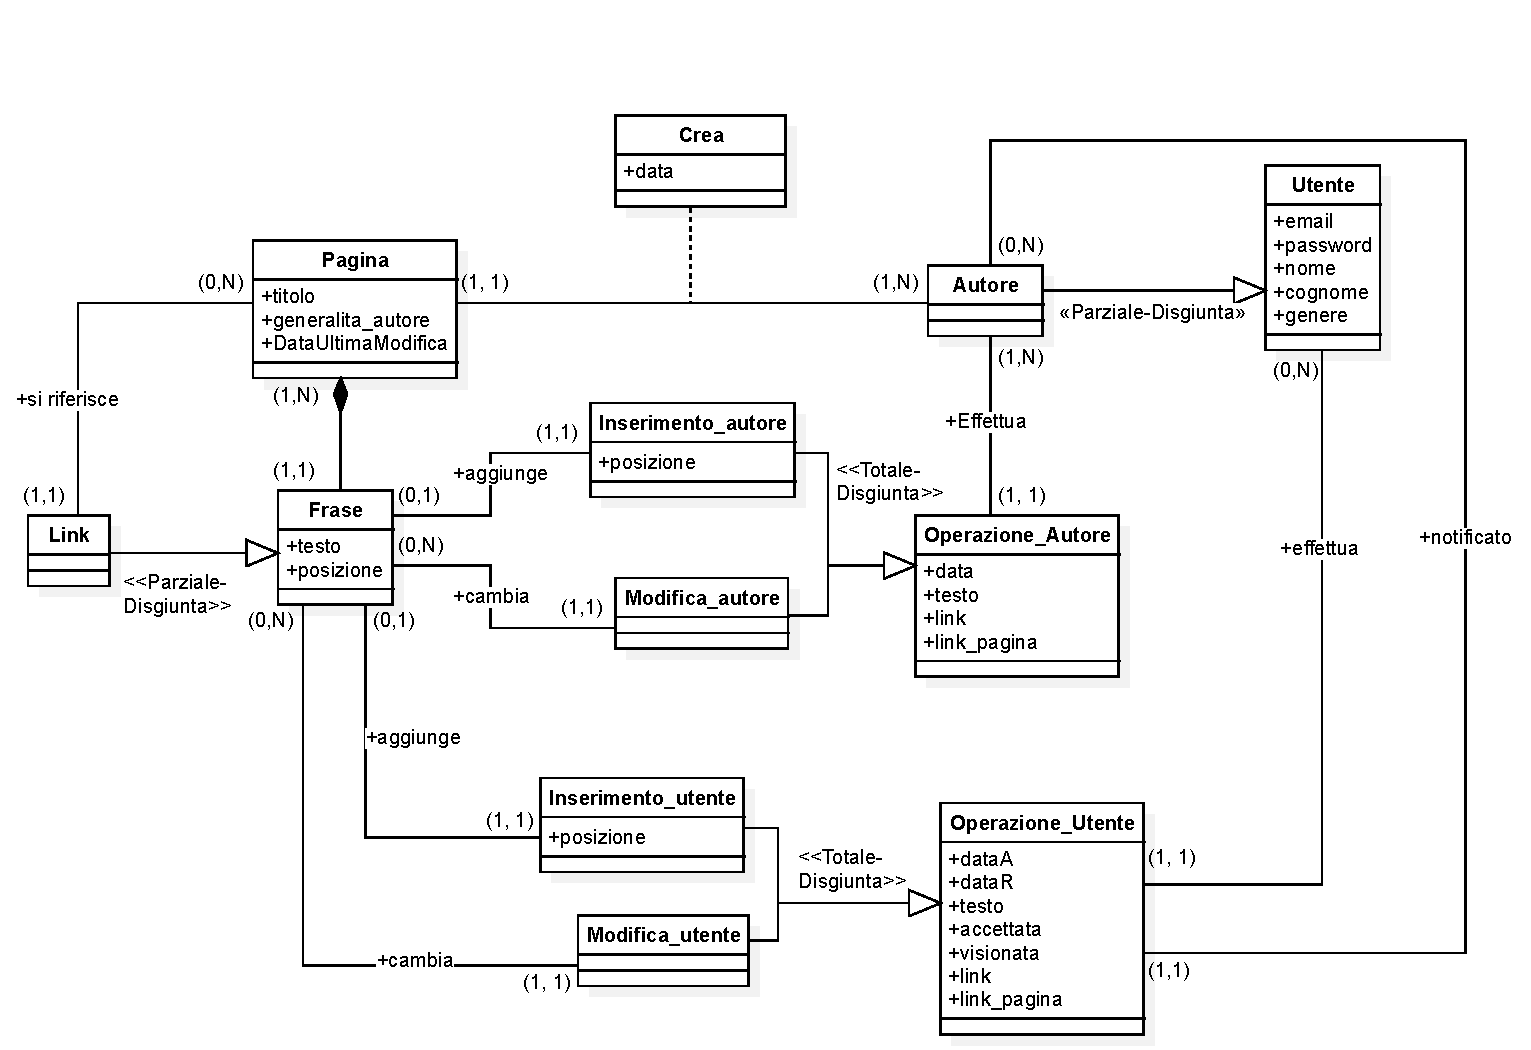
\includegraphics[width=1\textwidth]{Capitoli/Progettazione Concettuale/UML.pdf}
    %\caption{Descrizione dell'immagine}
    %\label{fig:nome_figura}
\end{figure}

\newpage
\subsection{Dizionario delle entità}
\input{Capitoli/Progettazione Concettuale/Dizionario delle entità}

\subsection{Dizionario delle associazioni}
\newcolumntype{L}{>{\raggedright\arraybackslash}p{4cm}}

\begin{longtable}{|p{3cm}|p{6cm}|L|}

\hline
\textbf{Associazioni} & \textbf{Descrizione} & \textbf{Attributi}\\
\hline

\endfirsthead
\multicolumn{3}{c}{} \\
\hline
\textbf{Associazioni} & \textbf{Descrizione} & \textbf{Attributi}\\
\hline
\endhead

Crea &  
Associazione \textbf{Molti-a-Uno} tra \textit{Pagina} e \textit{Autore}. Questa classe-associazione è utilizzata per memorizzare dati utili inerenti alla creazione della pagina. & 
\textbf{Data}(DateTime): Questo attributo si riferisce alla data di creazione della pagina wiki\\

\hline
Aggiunge (utente) & 
Associazione \textbf{Uno-a-Uno} tra \textit{Frase} e \textit{Inserimento utente}. Una farse può avere uno o zero inserimenti da parte del utente. Un' inserimento aggiunge una sola frase.
&\\

\hline
Cambia (utente)& 
Associazione \textbf{Molti-a-Uno} tra \textit{Frase} e \textit{Modifica utente}. Una frase può essere modificata zero o più volte. Una modifica può modificare solo una frase.
&\\

\hline
Aggiunge (autore)& 
Associazione \textbf{Uno-a-Uno} tra \textit{Frase} e \textit{Inserimento autore}. Una farse può avere uno o zero inserimenti da parte dell'autore. Un' inserimento aggiunge una sola frase.
&\\

\hline
Cambia (autore)& 
Associazione \textbf{Molti-a-Uno} tra \textit{Frase} e \textit{Modifica autore}. Una frase può essere modificata zero o più volte. Una modifica può modificare solo una frase.
&\\

\hline
Si riferisce &
Associazione \textbf{Molti-a-Uno} tra \textit{Link} e \textit{Pagina}. Questa associazione si riferisce al fatto che una frase (link) è collegata/contiene il collegamento ad un altra pagina wiki.&\\

\hline
Notificato &
Associazione \textbf{Molti-a-Uno} tra \textit{Operazione} e \textit{Autore}. Questa associazione si riferisce al fatto che un'autore visualizza le modifiche proposte alla sua pagina wiki. Una modifica verrà quindi visualizzata da un autore, ma l'autore visualizzerà tutte le modifiche inerenti alla sua pagina.&\\

\hline
Effettua&  
Associazione \textbf{Multi-a-Uno} tra \textit{Operazione} e \textit{Utente}. Questa associazione si riferisce al fatto che un utente ha la possibilità di proporre una frase alla pagina wiki. Un utente quindi può proporre nessuna o tante operazioni su una pagina, mentre un'operazione specifica di un utente è effettuata da un solo utente& \\

\hline
\end{longtable}

\newpage
\section{Ristrutturazione del modello concettuale}

\subsection{Analisi delle Ridondanze}
In questo fase analizzeremo le varie ridondanze e vedremo come gestirle
\subsubsection{Data ultima modifica}
\textit{data ultima modifica} è un attributo di pagina e potrebbe essere \textit{derivato}. Però essendo un informazione che deve essere reperita ogni volta che apriamo una pagina è conveniente averla subito disponibile e non  derivarla ogni volta.
Infatti se analizziamo la quantità di accessi ci converrà in grande scala non derivare la data di ultimo accesso. altrimenti dovremmo accedere ogni volta ad operazione utente e autore per capire chi è stato l'ultimo a fare una modifica. 

\subsubsection{Generalità\_Autore}
Questo attributo potrebbe essere derivato Notiamo che; le Generalità(Nome è cognome) del autore non cambiano molto spesso, quindi conviene per una questione di accessi creare un attributo apposito.

\subsection{Eliminazione delle Generalizzazioni}
In questa fase analizzeremo il tipo della generalizzazioni e come ristrutturarle

\subsubsection{Operazione utente e operazione autore}
    Operazione utente è una generalizzazione \textit{totale disgiunta} poiché un operazione è per forza al  più una modifica o un inserimento. Per una questione di accessi è molto meglio accorpare i figli nel padre. Questo perché in una situazione con un numero elevato di pagine potremmo avere di conseguenza tante richieste per la visione della storicità, modifiche proposte o proposte di inserimento. avremo in alcuni casi il doppio dei accessi o in altri casi il quadruplo dei accessi in più. Tutto questo può essere risparmiato accorpando i figli nel padre. Come contro avremo solo un \textit{attributo a null}, quest'ultimo è accettabile (attributo posizione potrà essere null) poiché aggiungendo questo valore a null ci risparmia molti accessi.\newline
    Operazione autore si elimina per lo stesso ragionamento e nello stesso metodo.
    
\subsubsection{Link}
    \textit{link} è una generalizzazione \textit{parziale/disgiunta} poiché una frase può non essere un link ma una frase non può essere altro oltre al link.
    Sempre per una questione di accessi conviene accorpare il \textit{padre} nei \textit{figli}. Questo perché ogni volta che carichiamo una wiki dobbiamo controllare anche se ci sono dei link. Accorpando il figlio nel padre avremo meno  accessi (uno in meno per controllare se una frase è un link e una in meno anche per navigare tra il link e la frase) velocizzando la risposta del database alla richiesta di visualizzazione di pagina. A discapito avremo un valore a \textit{null} se la frase non è un link. Anche se in un testo ci sono \textit{più frasi} che \textit{non sono un link} quindi i valori a null saranno \textit{consistenti}, Questo non ci interessa poiché è un male affrontabile  a noi interessa la \textit{velocità} con cui carichiamo una wiki.
    
\subsubsection{Autore}
    Un \textit{utente} è una generalizzazione \textit{parziale/disgiunta} poiché un utente può non essere un autore  ma una utente non può essere oltre che un autore.
    Sempre per una questione di accessi preferiamo inserire il figlio nel padre, questo ci permetterà di dimezzare gli accessi per capire chi è un autore. A discapito avremo un attributo che ci indicherà se un utente è un autore o meno. Ci saranno sicuramente più utenti che autori quindi potenzialmente ci potrebbero essere tanti valori a \textit{False(0)} ma il costo di questo attributo è di solo 1 bit. Otterremo sia meno accessi ma utilizzeremo più memoria rispetto a una diversa ristrutturazione ma la quantità di memoria utilizzata per salvare l'informazione sarà minima poiché l'attributo occupa solo un bit. Quindi se 300 utenti accedono avrò solo 300 accessi. Non avremo 600 accessi come nel caso di una diversa ristrutturazione; trasformazione della generalizzazione in relazioni. La ristrutturazione padre nel figlio a costo di accessi sarebbe stata uguale me non avrebbe avuto  molto senso a livello logico.

\subsection{Eliminazione degli attributi multivalore}
Non abbiamo valori multi valore 

\subsection{Eliminazione degli attributi composti}
Come valori composti abbiamo le date ma in questo caso  non ci servirà dividerle in ora e data. Per questo motivo le matteremo tutto nello stesso attributo

\subsection{Partizionamento/accorpamento di entità/associazioni}
Nessun accorpamento da fare
\subsection{Identificazione chiavi primarie}
\textbf{Utente} $\longmapsto$ Abbiamo scelto come chiave primaria \textit{Email}.\newline{}\newline{}
\textbf{Frase} $\longmapsto$ Non abbiamo nessuna chiave candidata però abbiamo una chiave parziale "\textit{posizione}". quest'ultimo insieme alla chiave esterna di \textit{Pagina} possiamo identificare univocamente una frase. questo perché in una pagina ci potrà essere solo una frase con la stessa posizione. La chiave primaria quindi è composta da \textit{chiave esterna} e \textit{posizione}\newline{}\newline{}
\textbf{Pagina} $\longmapsto$ il \textit{titolo} è una chiave candidata però per un questione di facilita di identificazione della pagina nella frase e anche per il link e meglio utilizzare una chiave auto incrementata di nome \textit{ID\_Pagina}\newline{}\newline{}
\textbf{Operazione\_Autore} $\longmapsto$ dipende sia da \textit{utente} che da \textit{frase} quindi essendo che non ci sono chiavi candidate e nemmeno chiave parziali invece di creare una chiave primaria molto grande raggruppando tutti gli attributi creeremo un codice di nome \textit{ID\_operazione} che si auto incrementa. Questo per facilitare l'accesso\newline{}\newline{}
\textbf{Operazione\_Utente} $\longmapsto$ dipende sia da \textit{utente} che da \textit{frase} quindi essendo che non ci sono chiave candidate e nemmeno chiave parziali invece di creare una chiave primaria molto grande raggruppando tutti gli attributi creeremo un codice di nome \textit{ID\_operazione} che si auto incrementa. Questo per facilitare l'accesso

\subsection{Schema Ristrutturato UML}
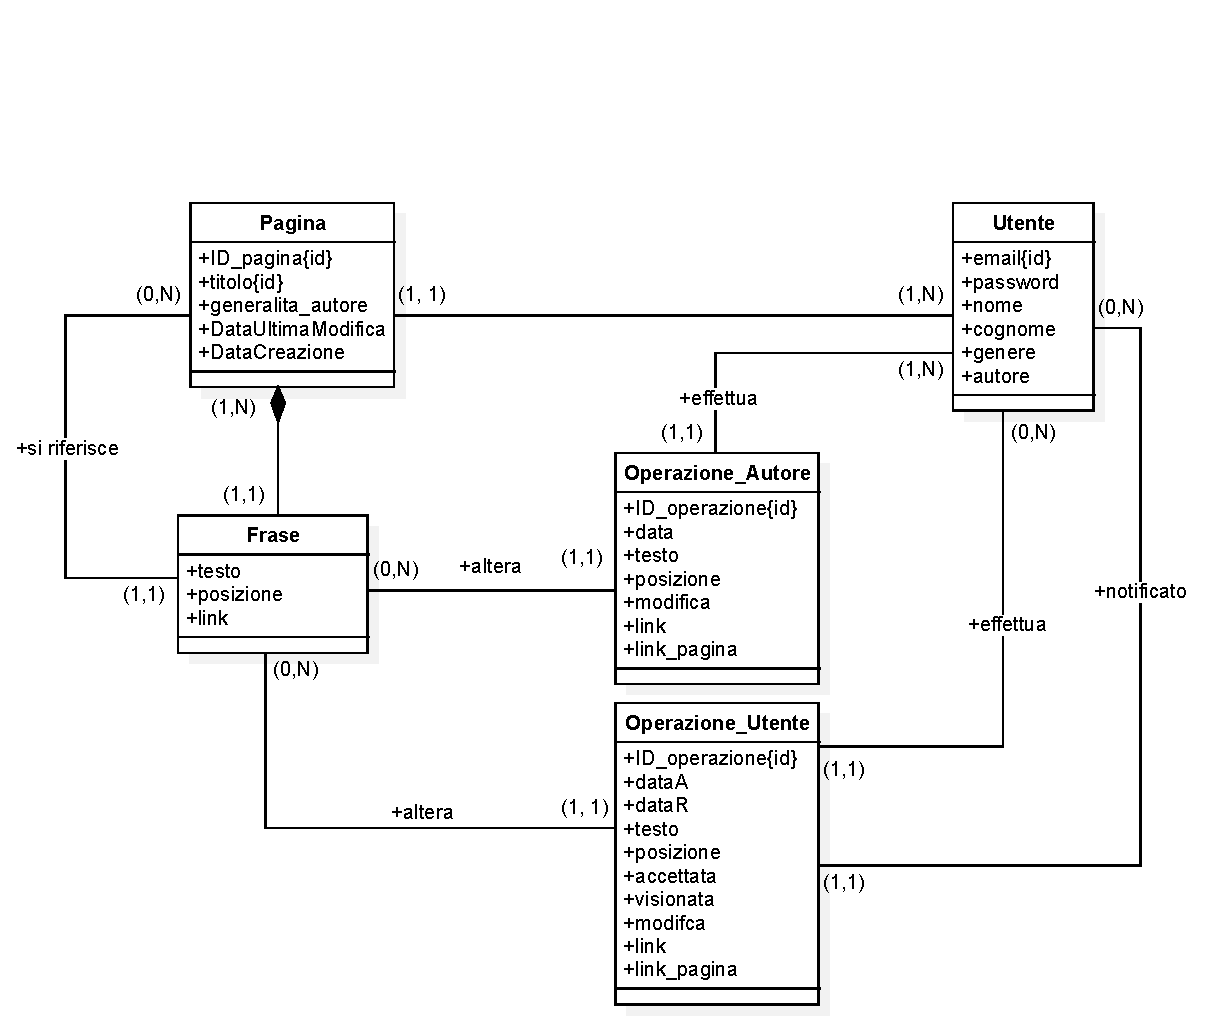
\includegraphics[width=1\textwidth]{Capitoli/Ristrutturazione/UML_Ristrutturato.pdf}

\subsection{Schema Ristrutturato ER}
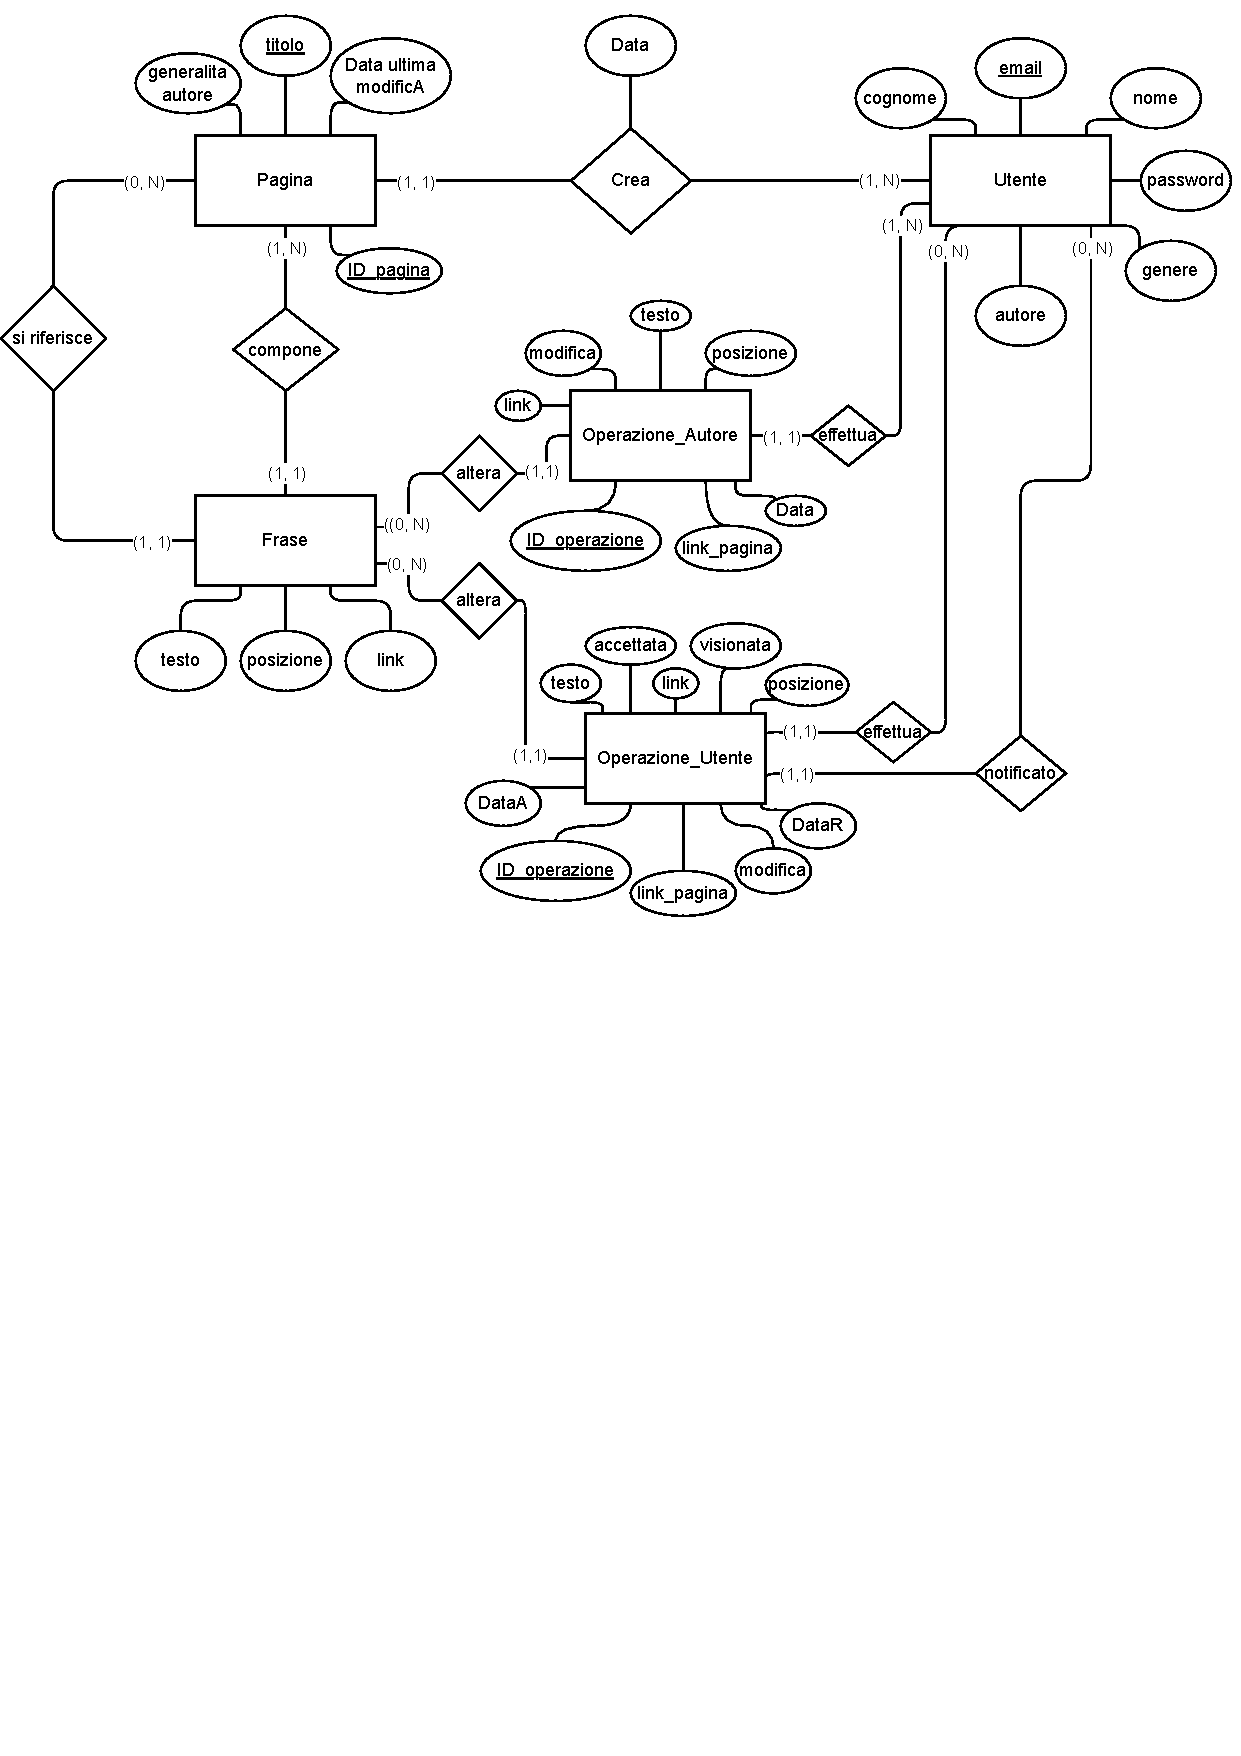
\includegraphics[width=1\textwidth]{Capitoli/Ristrutturazione/ER ristrutturato.pdf}

\newpage\newpage
\subsection{Dizionario delle Entità}
% Definizione di una nuova colonna per gli attributi con testo allineato a sinistra
%tabella associazioni
\newcolumntype{L}{>{\raggedright\arraybackslash}p{5cm}}

\begin{longtable}{|p{2.5cm}|p{6cm}|L|}

\hline
\textbf{Entità} & \textbf{Descrizione} & \textbf{Attributi} \\
\hline

\endfirsthead
\multicolumn{3}{c}{} \\
\hline
\textbf{Entità} & \textbf{Descrizione} & \textbf{Attributi} \\
\hline
\endhead

Utente & 
\textit{Utente} generico del sistema che può 
essere anche un autore di una pagina wiki &
\textbf{Nome}(String): Nome dell'utente \newline
\textbf{Cognome}(String): Cognome dell'utente \newline
\textbf{Email}(string): Email dell'utente \newline
\textbf{Password}(string): Password dell'utente \newline
\textbf{Genere}(Char): genere dell'utente \newline
\textbf{Autore}(Bit): Indica se l'utente è un autore (1) oppure un utente (0)\\

\hline
Pagina & L'entità pagina si riferisce alla \textit{pagina wiki} creata da un \textit{utente-autore} &
\textbf{ID\_Pagina}(Int): Numero intero auto incrementato che identifica univocamente una pagina dalle altre \newline
\textbf{Generalità autore}(String): Stringa composta dalle generalità  dell'autore della pagina \newline
\textbf{Titolo}(String): Indica il titolo della pagina, inoltre il titolo identifica univocamente una pagina dalle altre \newline
\textbf{Data ultima modifica}(Timestamp): Indica la data in cui è stata effettuata l'ultima modifica accettata sulla pagina 
\textbf{Data Creazione}(Timestamp): Indica la data in cui è stata effettuata la creazione della pagina\\

\hline
Frase & Frase è un elemento essenziale della pagina, perché una o più frasi
formano il testo della pagina &
\textbf{Testo}(String): Indica il contenuto testuale della frase \newline
\textbf{Posizione}(Int): Indica la posizione numerica all'interno della pagina \newline
\textbf{link}(Bit): questo attributo specifica se la frase è un collegamento ad un altra pagina se il valore è 1, se invece è 0 allora vuol dire che Frase non è un link\\

\hline
Operazione utente& 
Operazione utente è un entità \textit{Superclasse} che tiene traccia di tutte gli inserimenti e modifiche apportate, alle frasi di una pagina, dagli utenti, che esse siano accettate oppure no dall'autore della pagina &
\textbf{ID\_operazione}(String): Attributo auto incrementato che identifica l'operazione univocamente dalle altre\newline
\textbf{DataA}(Timestamp): Data in cui è stata accattata o rifiutata la modifica o inserimento dall'autore \newline
\textbf{DataR}(Timestamp): Data in cui è stata proposta la modifica o inserimento \newline
\textbf{Testo}(String): Contiene il testo inserito dall'utente \newline
\textbf{Accettata}(Bit): Indica se l'operazione proposta è stata accettata (1), rifiutata (0), il valore è inizializzato a 0 quando la proposta non è stata ancora accettata\newline
\textbf{Visionata}(Bit): Questo attributo indica se l'autore ha visionato (1) l'operazione oppure no (0) \newline
\textbf{Posizione}(Int): Posizione numerica specificata dall'utente al momento dell'inserimento di una nuova frase \newline
\textbf{Modifica}(Bit): Questo attributo indica se l'operazione è una modifica (1) oppure no (0)\newline
\textbf{link}(Bit): Indica se l'operazione è effettuata su un link (1) oppure no (0)\newline
\textbf{link\_pagina}(Int): Se l'operazione è effettuata su un link, questo attributo specifica a quale pagina la frase si riferisce\\

\hline
Operazione autore & 
Operazione autore è un entità \textit{Superclasse} che tiene traccia di tutte gli inserimenti e modifiche apportate, alle frasi di una pagina da parte dell'autore &
\textbf{ID\_operazione}(String): Attributo auto incrementato che identifica l'operazione univocamente dalle altre\newline
\textbf{Data}(Timestamp): Data in cui è stata apportata la modifica o inserimento \newline
\textbf{Testo}(String): Contiene il testo inserito dall'autore \newline
\textbf{Posizione}(Int): Posizione numerica specificata dall'autore al momento dell'inserimento di una nuova frase \newline
\textbf{Modifica}(Bit): Questo attributo indica se l'operazione è una modifica (1) oppure no (0)\newline
\textbf{link}(Bit): Indica se l'operazione è effettuata su un link (1) oppure no (0)\newline
\textbf{link\_pagina}(Int): Se l'operazione è effettuata su un link, questo attributo specifica a quale pagina la frase si riferisce\\

\hline
\end{longtable}

\newpage
\subsection{Dizionario delle associazioni}
\newcolumntype{L}{>{\raggedright\arraybackslash}p{4cm}}

\begin{longtable}{|p{3cm}|p{6cm}|L|}

\hline
\textbf{Associazioni} & \textbf{Descrizione} & \textbf{Attributi}\\
\hline

\endfirsthead
\multicolumn{3}{c}{} \\
\hline
\textbf{Associazioni} & \textbf{Descrizione} & \textbf{Attributi}\\
\hline
\endhead

Crea&  
Associazione \textbf{Molti-a-Uno} tra \textit{Pagina} e \textit{Autore}. Questa classe-associazione è utilizzata per memorizzare dati utili inerenti alla creazione della pagina.& 
\textbf{Data}(Timestamp): Questo attributo si riferisce alla data di creazione della pagina wiki.\\

\hline
Altera&
Associazione \textbf{Molti-a-Uno} tra \textit{Operazione Autore} e \textit{Frase}. Questa associazione si riferisce al fatto che una frase può subire modifiche oppure essere inserita in una pagina dall'autore&\\

\hline
Altera&
Associazione \textbf{Molti-a-UNo} tra \textit{Operazione Utente} e \textit{Frase}. Questa associazione si riferisce al fatto che una frase può subire modifiche oppure essere inserita in una pagina dall'utente, dopo l'approvazione dell'autore&\\

\hline
Si riferisce&
Associazione \textbf{Uno-a-Molti} tra \textit{Frase} e \textit{Pagina}. Questa associazione si riferisce al fatto che una frase (link) è collegata/contiene il collegamento ad un altra pagina wiki.&\\

\hline
Notificato&
Associazione \textbf{Molti-a-Uno} tra \textit{Operazione Utente} e \textit{Autore}. Questa associazione si riferisce al fatto che un'autore visualizza le modifiche proposte alla sua pagina wiki. Una modifica verrà quindi visualizzata da un autore, ma l'autore visualizzerà tutte le modifiche inerenti alla sua pagina.&\\

\hline
Effettua&  
Associazione \textbf{Molti-a-Uno} tra \textit{Operazione Utente} e \textit{Utente}. Questa associazione si riferisce al fatto che un utente ha la possibilità di proporre una frase alla pagina wiki. Un utente quindi può proporre nessuna o tante operazioni su una pagina&\\

\hline
Effettua&  
Associazione \textbf{Molti-a-Uno} tra \textit{Operazione Autore} e \textit{Utente}. Questa associazione si riferisce al fatto che un autore ha la possibilità la pagina wiki attraverso le operazioni sulle frasi. Un autore quindi può proporre nessuna o tante operazioni su una pagina ma effettuerà come minimo un'inserimento&\\

\hline
\end{longtable}


\newpage
\section{Traduzione al Modello Logico}

\subsection{Mapping delle Associazioni}
\subsubsection{Associazioni 1-N o N-1}
\begin{itemize}
    \item{\textbf{Autore - Crea - Pagina}, Inseriamo la chiave di Autore come chiave esterna di pagina}\newline
    \item{\textbf{Operazione Autore - Altera - Frase}, aggiungiamo la chiave di frase come chiave estera in Operazione Autore}\newline
    \item{\textbf{Operazione Utente - Altera - Frase}, aggiungiamo la chiave di Frase come chiave estera in Operazione Utente}\newline
    \item{\textbf{Frase - Si riferisce - Pagina},
    inseriamo la chiave di pagina come chiave sterna di frase}\newline
    \item{\textbf{Operazione Utente - Notifica - Autore}, inseriamo la chiave di Autore come chiave esterna di Operazione Utente}\newline
    \item{\textbf{Utente  - Effettua - Operazione utente}, inseriamo la chiave di Utente come chiave esterna di Operazione Utente}\newline
    \item{\textbf{Autore  - Effettua - Operazione Autore}, inseriamo la chiave di Autore come chiave esterna di Operazione Autore}\newline
\end{itemize}

\subsubsection{Associazioni N-N}
Non sono presenti relazioni N-N
\newpage

\subsection{Modello logico}
Gli attributi \underline{sottolineati} sono chiavi primarie.\newline
Gli Attributi in \textbf{MAIUSCOLO} sono chiavi esterne.\newline
Gli Attributi con * possono essere NULL
\newline\newline
\textbf{Utente}(\underline{Email}, Nome, Password, Genere, Autore)\newline\newline
\textbf{Pagina}(\underline{ID\_Pagina}, Titolo, Nome\_autore, DataUltimaModifica, Data Creazione, \textbf{AUTORE})\newline
\textit{Pagina.AUTORE} $\longmapsto$ \textit{Utente.Email}
\newline\newline
\textbf{Frase}(\underline{Posizione, \textbf{PAGINA}}, Testo, Link, \textbf{LINKPAGINA}*)
\newline
\textit{Frase.PAGINA} $\longmapsto$ \textit{pagina.ID\_pagina}
\newline
\textit{Frase.LINKPAGINA} $\longmapsto$ \textit{pagina.ID\_pagina}
\newline\newline
\textbf{Operazione Autore}(\underline{ID\_Operazione}, Data, Testo, PosizioneIns*, Modifica, link, link\_pagina*, \textbf{FRASE}, \textbf{AUTORE})\newline
\textit{Operazione Utente.FRASE} $\longmapsto$ \textit{Frase.(Posizione,PAGINA)}\newline
\textit{Operazione Autore.AUTORE} $\longmapsto$ \textit{Utente.Email}
\newline\newline
\textbf{Operazione Utente}(\underline{ID\_Operazione}, DataA*, DataR, Testo, PosizioneIns*, link, link\_pagina*, Accettata, Visionata, Modifica, \textbf{FRASE}, \textbf{UTENTE}, \textbf{AUTORE\_NOTIFICATO})\newline
\textit{Operazione Utente.FRASE} $\longmapsto$ \textit{Frase.(Posizione*,PAGINA)}\newline
\textit{Operazione Utente.UTENTE} $\longmapsto$ \textit{Utente.Email}
\newline
\textit{Operazione Utente.AUTORE\_NOTIFICATO} $\longmapsto$ \textit{Utente.Email}
\newpage

\section{Progettazione Fisica}

\subsection{Creazione delle tabelle}
\lstinputlisting{Capitoli/Progettazione Fisica/creazione delle tabelle.txt}
\newpage

\subsection{Vincoli}
Identifichiamo in questa sezione i vincoli legati al nostro dominio

\subsubsection{Vincoli di Domino}
\begin{itemize}

    \item {
        \textbf{d\_Email} è un dominio che controlla se un email è valida o  meno. Questo dominio non è totale, ci potrebbero essere altri problemi come; doppia chioccola o doppio punto. L'Email dovrà essere comunque controllata, tutta via questo check eviterà lavoro superfluo al trigger che avrà il compito di controllare Email al momento del inserimento\newline
        \lstinputlisting{Capitoli/Progettazione Fisica/domini.sql}
    }
    \item {\textbf{CheckGenere} Limita il campo dei VARCHAR a due solo valori 'F' o 'M', creando un dominio formato solo da 'F' o 'M'}
    
    
\end{itemize}

\subsubsection{Vincoli sui valori NULL e valori predefiniti}
\begin{itemize}
    \item{Tutti i valori non possono essere NULL escludendo:
        \begin{itemize}
            \item{\textbf{dataA} data Accettazione o Rifiuto dell'operazione}
            \item{\textbf{LINKPAGINA} cioè il riferimento a una pagina tramite un link}
            \item{\textbf{posizione\_frase} è il riferimento alla frase in operazione utente. quest'ultimo può essere null poiché quando faremo una richiesta di inserimento la frase non esiste}
            \item{\textbf{posizioneIns} è la posizione di inserimento della frase, se L'operazione è una modifica questo valore sarà NULL}
        \end{itemize}
    }
    \item{Non ci sono valori Default}
\end{itemize}

\subsubsection{Identificazione vincoli intrarelazionali}

\textbf{Vincoli di Chiave:}
\begin{itemize}
    \item {Sono tutte le chiavi primarie nelle rispettive relazioni.}\newline
\end{itemize}
\textbf{Vincoli di Tupla:}
\begin{itemize}
    \item {se l'attributo \textit{"link"} in \textit{"Operazione Utente"} e in \textit{"Operazione Autore"} è impostato a \textit{True} allora \textit{"link\_pagina"} non dovrà essere NULL (costrain di nome \textbf{CheckLink})}
    
\end{itemize}

\subsubsection{Identificazione vincoli interrelazionali}
\textbf{Vincoli di integrità referenziale:}
\begin{itemize}

    \item {Se la Chiave primaria di una \textit{"pagina"} viene modificata allora anche i riferimenti devono essere aggiornati}
    \item {Se la Chiave primaria di un'\textit{"utente"} viene modificata allora anche i riferimenti devono essere aggiornati}
    \item {Se un \textit{"link"} fa riferimento ad una \textit{"pagina eliminata"}, allora il link non deve contenere nessun riferimento (NULL)}
    \item {Quando viene eliminata una \textit{"pagina"}, deve essere eliminato tutto il suo contenuto (Frasi), le sue occorrenze e le occorrenze del contenuto (Operazioni Utente e Autore)}\newline
\end{itemize}
\textbf{Vincoli di integrità semantica:}
\begin{itemize}
    
    \item {Se l'attributo\textit{"visionata"} in \textit{"Operazione Utente"} è impostato a \textit{True} allora l'utente non potrà modificare quella proposta. \hyperlink{Modificaproposta}{\textbf{Clica qui}}}\newline
    
    \item {Un \textit{"Utente"} non può essere cancellato.  \hyperlink{UtenteNoDelete}{\textbf{Clica qui}}}\newline
    
    \item {Un \textit{"Utente"} Diventa autore se crea una pagina. \hyperlink{SwitchAutore}{\textbf{Clica qui}}}\newline

    \item {Un \textit{"Autore"} Diventa Utente se non ha più nessuna pagina. \hyperlink{SwitchUtente}{\textbf{Clica qui}}}\newline
    
    \item { In \textit{"Pagina"} deve essere aggiornato il valore di Generalità\_autore in caso di modifica delle generalità dell'autore. \hyperlink{AggiornamentoGeneralitaPagina}{\textbf{Clica qui}}}\newline
    
    \item {La \textit{"DataR"} deve combaciare sempre con l'ultima Data di modifica del testo. \hyperlink{ModificaDataMod}{\textbf{Clica qui}}}\newline
    
    \item {Una \textit{"Pagina"} non può essere vuota.  \hyperlink{CreazionePagina}{\textbf{Clica qui}}}\newline

    \item {\textit{"DataUltimaModifica"} in "Pagina" deve essere aggiornata quando viene aggiunta o modificata una frase nella pagina. \hyperlink{DataModficaPagina}{\textbf{Clica qui}}}\newline
    
    \item {Le azioni dell'autore sono registrate in \textit{Operazione\_autore}. \hyperlink{OperazioneAutoreIntegritaMod}{\textbf{Clica qui}} e  \hyperlink{OperazioneAutoreIntegritaIns}{\textbf{Clica qui}}}\newline
    
    \item {Le azioni dell'utente sono registrate in \textit{Operazione\_utente}. \hyperlink{OperazioneUtenteRichiesta}{\textbf{Clica qui}}}
\end{itemize}

\newpage
\subsection{Trigger}
\lstset{
    language=SQL, 
    basicstyle=\small\ttfamily,
    numbers=left, 
    numberstyle=\tiny, 
    frame=line,
    keywordstyle=\color{blue},
    commentstyle=\color{red},
    stringstyle=\color{red},
    identifierstyle=\color{black},
    numberstyle=\tiny\color{black},
    breaklines=true,
    linewidth=1.2\linewidth,
    showstringspaces=false,
}

\hypertarget{Modificaproposta}{}
\subsubsection{Modifica\_proposta}
\textbf{Vincolo}: Se l'attributo\textit{"visionata"} in \textit{"Operazione Utente"} è impostato a \textit{True} allora l'utente non potrà modificare quella proposta\newline\newline
\textbf{Descrizione}: è un \textit{trigger} che al  momento della modifica del \textit{testo} in \textit{operazione\_utente}, prima di inserire la tupla controlla se quella "proposta di modifica" è stata già visualizzata. Se visionata è \textit{True(1)} allora impedisce l'Inserimento con un Excption.\newline

\lstinputlisting{Capitoli/Progettazione Fisica/Trigger/Trigger Modifica_proposta.txt}


\hypertarget{UtenteNoDelete}{}
\subsubsection{Utente\_No\_Delete}
\textbf{Vincolo}: Un \textit{"utente"} non può essere cancellato\newline\newline
\textbf{Descrizione}: Lancia un'eccezione prima che una tupla nella tabella \textit{utente} venga cancellata.\newline

\lstinputlisting{Capitoli/Progettazione Fisica/Trigger/Trigger Utente_No_Delete.txt}


\hypertarget{ModificaDataMod}{}
\subsubsection{ModificaDataMod}
\textbf{Vincolo}: La \textit{DataR} deve combaciare sempre con l'ultima Data di modifica del testo\newline\newline
\textbf{Descrizione}: Il \textit{"set time zone 'Europe/Rome';"} serve per impostare l'ora italiana. Questo trigger si occuperà di Modificare DataR nella data in cui è stato fatto l'Ultimo cambiamento al testo. \newline
\lstinputlisting{Capitoli/Progettazione Fisica/Trigger/ModificaDataMod.txt}

\newpage
\hypertarget{AggiornamentoGeneralitaPagina}{}
\subsubsection{Aggiornamento\_Generalita\_Pagina}
\textbf{Vincolo}: In \textit{"pagina"} deve essere aggiornato il valore di Generalità\_autore in caso di modifica delle generalità dell'autore. \newline\newline
\textbf{Descrizione}: Questo trigger prenderà tutte le pagine con l'email dell'autore a cui sono state aggiornate le generalità. Dopodiché prende il nome e il cognome aggiornati e li separa da un "\textbf{;}" poiché un nome o un cognome potrebbero avere spazzi. Per ogni pagina dell'autore aggiorneremo le generalità con le informazioni aggiornate.\newline
\lstinputlisting{Capitoli/Progettazione Fisica/Trigger/Trigger Aggiornamento_Generalita_Pagina.txt}

\newpage
\hypertarget{SwitchAutore}{}
\subsubsection{SwitchAutore}
\textbf{Vincolo}: Un \textit{"Utente"} Diventa autore se crea una pagina \newline\newline
\textbf{Descrizione}: Dopo aver inserito una pagina controlliamo se l'utente che ha creato la pagana è già un autore. Nel caso non lo fosse allora aggiorniamo il parametro autore a \textit{True}.
\lstinputlisting{Capitoli/Progettazione Fisica/Trigger/SwitchAutore.txt}


\hypertarget{SwitchUtente}{}
\subsubsection{SwitchUtente}
\textbf{Vincolo}: Un \textit{"Autore"} Diventa Utente se non ha più nessuna pagina \newline\newline
\textbf{Descrizione}: dopo la cancellazione di una pagina controlliamo se l'autore della pagina cancellata ha altre pagine. se la query restituisce qualcosa allora non faremo nulla altrimenti l'autore diventerà Utente.\newline
\lstinputlisting{Capitoli/Progettazione Fisica/Trigger/SwitchUtente.txt}

\newpage
\hypertarget{DataModficaPagina}{}
\subsubsection{DataModficaPagina}
\textbf{Vincolo}: \textit{"DataUltimaModifica"} in \textit{"Pagina"} deve essere aggiornata quando viene aggiunta o modificata una frase nella pagina. \newline\newline
\textbf{Descrizione}: Quando inserisco o modifico in \textbf{frase} significa che ho modificato la pagina. Quindi aggiorno la \textit{"DataUltimaModifica"} della pagina.\newline
\lstinputlisting{Capitoli/Progettazione Fisica/Trigger/DataModficaPagina.txt}


\hypertarget{OperazioneAutoreIntegritaIns}{}
\subsubsection{OperazioneAutoreIntegritaIns}
\textbf{Vincolo}: Le azioni dell'autore sono registrate in \textit{Operazione\_autore}\newline\newline
\textbf{Descrizione}: Quando un autore inserisce una frase l'operazione verrà registrata nei \textbf{LOG} dell'autore.\newline
\lstinputlisting{Capitoli/Progettazione Fisica/Trigger/Operazione Autore Integrita Ins.txt}


\hypertarget{OperazioneAutoreIntegritaMod}{}
\subsubsection{OperazioneAutoreIntegritaMod}
\textbf{Vincolo}: Le azioni dell'autore sono registrate in \textit{Operazione\_autore}\newline\newline
\textbf{Descrizione}: Quando un autore modifica una frase l'operazione verrà registrata nei \textbf{LOG} dell'autore.\newline
\lstinputlisting{Capitoli/Progettazione Fisica/Trigger/Operazione Autore integrita Mod.txt}

\newpage
\subsubsection{PositionControll}
\textbf{Scopo}: Permette l'inserimento e  ottimizza l'inserimento. Si creano dei intervalli tra le parole per permettere di inserire nel mezzo senza spostare tutte le frasi.\newline\newline
\textbf{Descrizione}: Questo trigger viene attivato ogni volta che viene inserita una frase in una pagina. Esso controlla la posizione massima (La posizione dell'ultima frase), se esiste l'immagazzina in una variabile(max\_pos) altrimenti imposta la variabile a zero (max\_pos). se la posizione massima (max\_pos) è più piccola della posizione di inserimento (new.posizione) allora creo un intervallo tra max\_pos e la nuova posizione della parola, questo perché se voglio inserire nel mezzo non troverò difficoltà. Nel caso opposto (max\_pos maggiore uguale a new.posizione) controlliamo prima se la nuova posizione è \textit{"1"} poiché è un caso particolare (ovvero se si inserisce una frase in testa, allora devo spostare tutte le frasi). Altrimenti imposto la nuova posizione (new.posizione) a meta dell'intervallo (tra il più piccolo dei successori e il più grande dei predecessori). Se questa posizione già esiste (caso in cui lo spazio tra due frasi è terminato) allora chiamo \hyperlink{UpadatePosition}{\textbf{UpadatePosition}} (che aggiunge spazzino nel'intervallo). In fine \textit{new.posizione} sarà impostata a meta del nuovo intervallo.\newline
\lstinputlisting{Capitoli/Progettazione Fisica/Trigger/Position Controll.txt}

\newpage
\subsubsection{CheckAggiornamentoPagina}
\textbf{Scopo}: Inserisce/modifica le frasi accettate dall'autore nelle pagine corrispondenti.\newline\newline
\lstinputlisting{Capitoli/Progettazione Fisica/Trigger/CheckAggiornamentoPagina.txt}

\subsubsection{DeleteFraseOpUtente}
\textbf{Implementazione di}: \textit{Quando viene eliminata una ”pagina”, deve essere eliminato tutto il suo contenuto (Frasi), le sue occorrenze e le occorrenze del contenuto (Operazioni Utente e Autore)}.\newline\newline
\textbf{Descrizione}: Questo trigger serve per eliminare le occorrenze di proposte di inserimento quando una pagina viene eliminata.\newline
\lstinputlisting{Capitoli/Progettazione Fisica/Trigger/DeleteFraseOpUtente.txt}

\newpage
\subsection{Funzioni e Procedure}
\hypertarget{CreazionePagina}{}
\subsubsection{CreazionePagina}
\textbf{Vincolo}: Una \textit{"Pagina"} non può essere vuota \newline\newline
\textbf{Descrizione}: Si potrà creare una pagina solo tramite questa Procedura. Inoltre la procedura garantirà che subito dopo alla creazione di una pagina ci sarà un inserimento di una frase. Essendo tutta la Procedura in un blocco \textbf{BEGIN/END} nel caso ci fosse un errore sarà fatto il \textbf{ROLLBACK} cosi mantenendo la \textit{consistenza nel DB}.\newline
\lstinputlisting{Capitoli/Progettazione Fisica/Funzioni/Creazione Pagina.txt}

\newpage
\subsubsection{InsertFraseAutore}
\textbf{Scopo}: Inserire una frase \newline\newline
\textbf{Descrizione}: La Procedura controlla che l'utente inserito esiste, controlla se la frase che stiamo inserendo deve diventare un link e controlla se la pagina a cui fa riferimento il link esiste. Dopodiché inseriamo la frase. Se la frase non è link inseriamo senza mettere riferimenti ad altre pagine. \newline
\lstinputlisting{Capitoli/Progettazione Fisica/Funzioni/inserimento frase autore.txt}

\newpage
\subsubsection{ModificaFraseAutore}
\textbf{Scopo}: Premete la modifica di una frase da parte dell'autore della pagina \newline\newline
\textbf{Descrizione}: La Procedura controlla che l'utente inserito esiste, se la frase che stiamo modificando deve diventare un link e se la pagina a cui fa riferimento il link esiste. Dopodiché modifichiamo la frase. se la frase non è link modifichiamo solo il testo.\newline
\lstinputlisting{Capitoli/Progettazione Fisica/Funzioni/modifica frase autore.txt}

\newpage
\subsubsection{CheckAutore}
\textbf{Scopo}: Funzione che controlla se le operazioni sono concrete e svolte dall'autore della pagina.\newline\newline
\textbf{Descrizione}: Questa procedura permette di controllare le seguiteti condizioni: se la pagina inserita esiste, se l'utente inserito esiste ed è autore e se la pagina su cui vogliamo applicare la modifica è effettivamente la nostra. Se una di queste condizioni non è vera allora verrà lanciato un \textbf{EXCETION}.\newline
\lstinputlisting{Capitoli/Progettazione Fisica/Funzioni/Check Autore.txt}

\newpage
\hypertarget{OperazioneUtenteRichiesta}{}
\subsubsection{OperazioneUtenteRichiesta}
\textbf{Vincolo}: Le azioni dell'utente sono registrate in \textit{Operazione\_utente} \newline\newline
\textbf{Descrizione}: Questa funzione permette al utente di richiedere un inserimento o una modifica. in base ai parametri inseriti andremo nel caso del inserimento o della modifica. Sempre tramite parametri possiamo capire se vogliamo che quella frase diventi/sia un link\newline
\lstinputlisting{Capitoli/Progettazione Fisica/Funzioni/OperazioneUtenteRichiesta.txt}

\newpage
\subsubsection{GetUserModPage}
\textbf{Scopo}: Lista di tutti gli utenti che hanno almeno una volta proposto un operazione su almeno una pagina dell'autore in input oppure una Lista di utenti che hanno almeno una volta proposto un operazione su una pagina in input e su un autore specifico. \newline\newline
\textbf{Descrizione}: Utilizzeremo SQL dinamico per creare la query. Se l'input della pagina (paginaIn) sarà \textit{'0'} Allora la funzione ritorna tutte gli utenti che hanno Richiesto un Operazione su almeno una pagina dell'autore che richiama la funzione. Quindi tramite un cursore scorro tutte le pagine dell'autore e le aggiungo alla condizione della query. Altrimenti aggiungo solo la pagina interessata. La funzione restituisce una stringa dove ogni utente e diviso tramite un \textit{';'}
\lstinputlisting{Capitoli/Progettazione Fisica/Funzioni/GetUserModPage.txt}


\newpage
\hypertarget{UpadatePosition}{}
\subsubsection{UpadatePosition}
\textbf{Scopo}: Aggiorna la posizione da un certo valore. Aggiorna i valori dal più grande al più piccolo\newline\newline
\textbf{Descrizione}: Questa funzione dato la pagina (pagina\_in) la posizione (posizione\_in) e il caso aggiornerà tutte le posizioni che sono maggiori della posizione\_in nel caso diverso da 1 (caso != 1) altrimenti quelli maggiori uguali. Questo perché 1 è un caso particolare e deve essere gestito singolarmente.\newline
\lstinputlisting{Capitoli/Progettazione Fisica/Funzioni/UpadatePosition.txt}

\newpage
\subsubsection{AccettaProposta}
\textbf{Scopo}: Procedura che permetta all'autore di accettare o rifiutare una proposta di modifica da parte di un utente.\newline\newline
\textbf{Descrizione}:La procedura andrà a registrare nel LOG di operazione\_utente la data di accettazione/rifiuto e setterà l'attributo accettata a True. L'inserimento o l'aggiornamento delle modifiche di una frase sarà fatto da un trigger.\newline
\lstinputlisting{Capitoli/Progettazione Fisica/Funzioni/AccettaProposta.txt}


\newpage
\subsubsection{GetLimtUserModPage}
\textbf{Scopo}: Ci permette di vedere tutti gli utenti che hanno proposto almeno una volta una modifica/inserimento rispetto a una serie di pagine in input.\newline\newline
\textbf{Descrizione}: La funzione prenderà in input una stringa contente una serie di Id\_pagina divisi da un \textit{'+'}. Tramite sql dinamico creiamo una query che selezionerà tutti gli utenti che hanno almeno proposto una modifica/inserimento nelle pagine in input. Dopodiché aver preso tutte l'email distinte fra di loro  inseriamo ogni email in una stringa di output, dove ogni email è diviso da un \textit{'+'}.\newline
\lstinputlisting{Capitoli/Progettazione Fisica/Funzioni/GetLimtUserModPage.txt}

\newpage
\subsubsection{VisualizzaPropostaAndConfronta}
\textbf{Scopo}: Funzione che permettere di visualizzare i dati di un inserimento e confrontare i dati tra una frase e la sua proposta di modifica.\newline\newline
\textbf{Descrizione}: La funzione verifica che l'id dell'operazione passata esiste, se l'utente che sta visualizzando l'operazione ha diritto a visualizzare la notifica e se è autore della pagina in cui è stata effettuata la proposta. Superati i controlli nel caso dell'inserimento la funzione restituisce una stringa, contente i dati della frase che l'utente vuole inserire, cosi formattata:  \textbf{'titolo+testo,posizione,link,id\_pagina\_riferita,titolo\_pagina\_riferita'}. Nel caso di una modifica verranno confrontati i dati originali con quelli proposti, e la stringa restituita sarà cosi formattata: \textbf{'Titolo+testo, posizione,link, id\_pagina\_riferita, titolo\_pagina\_riferita; proposta\_testo, proposta\_posizione, proposta\_link, proposta\_id\_pagina\_riferita, proposta\_titolo\_pagina\_riferita'}.\newline
\lstinputlisting{Capitoli/Progettazione Fisica/Funzioni/visualizzaPropostaAndConfronta.txt}

\newpage
\subsubsection{trovaPagina}
\textbf{Scopo}: Permette di cercare le pagine wiki.\newline\newline
\textbf{Descrizione}: Una volta passata la stringa di ricerca/input la funzione andrà a cercare tutte le pagine che contengono nel titolo le stesse parole e ritornerà una stringa cosi formattata \textbf{'id1-id2-...-idn'} contenente gli id delle pagine che corrispondono alla ricerca. Se nessuna pagina viene trovata allora la funzione ritornerà \textbf{'-1'}.
\lstinputlisting{Capitoli/Progettazione Fisica/Funzioni/trovaPagine.txt}


\subsubsection{ModificaRichestaProposta}
\textbf{Scopo}: Permette di modificare una proposta inviata.\newline\newline
\textbf{Descrizione}: La procedura controlla se esiste la proposta del utente. Se esiste modifica il testo altrimenti lancia un \textbf{EXCEPTION}.
\lstinputlisting{Capitoli/Progettazione Fisica/Funzioni/ModificaRichestaProposta.txt}

\newpage
\subsection{Viste}
\lstset{
    language=SQL, 
    basicstyle=\small\ttfamily,
    numbers=left, 
    numberstyle=\tiny, 
    frame=line,
    keywordstyle=\color{blue},
    commentstyle=\color{red},
    stringstyle=\color{red},
    identifierstyle=\color{black},
    numberstyle=\tiny\color{black},
    breaklines=true,
    linewidth=1.2\linewidth,
    showstringspaces=false,
}

\subsubsection{Storicita\_totale}
\textbf{Implementazione di}:  \textit{Tutti gli autori potranno vedere tutta la storia di tutti i testi dei quali sono autori e di tutti quelli nei quali hanno proposto una modifica.}
\newline
\lstinputlisting{Capitoli/Progettazione Fisica/view/Storicita totale.txt}

\subsubsection{Notifica}
\textbf{Implementazione di}: \textit{La modifica proposta verrà notificata all’autore del testo originale la prossima volta che utilizzerà il sistema}.
\newline\newline
\textbf{Descrizione}: Vista che contiene tutte le notifiche di tutti gli autori che hanno una proposta di modifica ancora non accettata/rifiutata. Questa vista è utile per ottenere tutte le informazioni riguardanti le proposte in corso, per questo è preferibile una vista anziché una funzione funzione che faccia la stessa cosa filtrando per autore.
\lstinputlisting{Capitoli/Progettazione Fisica/view/Notifica.txt}

\newpage
\subsubsection{Log\_page}
\textbf{Implementazione di}: \textit{Tutti gli autori potranno vedere tutta la storia di tutti i testi dei quali sono autori}.
\newline\newline
\textbf{Descrizione}: Questa vista permette di vedere la storicità di tutti i testi ordinati per pagina e data.
\lstinputlisting{Capitoli/Progettazione Fisica/view/log_page.txt}

\newpage
\section{Dizionari degli Errori}
\begin{enumerate}[label=\textbf{\arabic*.}]
    \item '\textcolor{red}{E01}: Non esiste una proposta per $<$email-autore$>$ con id\_operazione $<$id-operazione$>$'\newline\newline
    \textbf{Descrizione}: Eccezione lanciata dalla procedura AccettaProposta, quando l'autore tenta di accettare una proposta di operazione che non esiste oppure che non deve essere accettata da quell'autore.

    \item '\textcolor{red}{E02}: Questo utente non e autore della pagina'\newline\newline
    \textbf{Descrizione}: Eccezione lanciata dalla procedura CheckAutore, quando un utente-autore non è autore della pagina su cui si sta effettuando delle operazioni.
    
    \item '\textcolor{red}{E03}: Utente non trovato o utente non e autore'\newline\newline
    \textbf{Descrizione}: Eccezione lanciata dalla procedura CheckAutore, quando si sta esaminando l'operazione da effettuare e risulta che l'utente-autore che sta effettuando l'operazione non esiste oppure non è un autore.
    
    \item '\textcolor{red}{E04}: La pagina non esiste (link non valido)'\newline\newline
    \textbf{Descrizione}: Eccezione lanciata dalle procedure:
    \begin{itemize}
        \item InsertFraseAutore
        \item OperazioneUtenteRichiesta
    \end{itemize}
    quando si sta esaminando l'operazione da effettuare e risulta che la pagina a cui il link fa riferimento non esiste.
    
    \item '\textcolor{red}{E05}: Utente non trovato'\newline\newline
    \textbf{Descrizione}: Eccezione lanciata dalla procedura CreazionePagina, quando l'utente che sta creando la pagina non corrisponde ad un utente registrato nel database

    \item '\textcolor{red}{E06}: utente non può essere cancellato'\newline\newline
    \textbf{Descrizione}: Eccezione lanciata dal trigger Utente\_No\_Delete, quando si effettua una qualunque operazione di cancellazione di un utente
    
    \item '\textcolor{red}{E07}: La modifica e gia stata visionata'\newline\newline
    \textbf{Descrizione}: Eccezione lanciata dal trigger Modifica\_proposta, quando un utente sta tentando di modificare una proposta di modifica, ma l'autore ha già visionato la proposta.

    \item '\textcolor{red}{E08}:La frase non esiste'\newline\newline
    \textbf{Descrizione}: Eccezione lanciata dalla procedura OperazioneUtenteRichiesta quando si tenta di proporre una modifica ad una frase che non esiste.

    \item '\textcolor{red}{E09}:La pagina non esiste' \newline\newline
    \textbf{Descrizione}: Eccezione lanciata dalle Procedure:
    \begin{itemize}
        \item OperazioneUtenteRichiesta
        \item CheckAutore
    \end{itemize}
    quando si tenta di inserire/proporre una frase in una pagina che non esiste.

    \item '\textcolor{red}{E10}: Utente non corretto' \newline\newline
    \textbf{Descrizione}: Eccezione lanciata dalla procedura OperazioneUtenteRichiesta quando l'utente che sta effettuando l'operazione non esiste.

    \item '\textcolor{red}{E11}: l''autore inserito non e autorizzato a visualizzare questa notifica'\newline\newline
    \textbf{Descrizione}: Eccezione lanciata dalla funzione visualizzaPropostaAndConfronta quando l'autore che sta tentando di visualizzare le proposte di modifica non è lo stesso autore della pagina in cui è stata effettuata la proposta.

    \item '\textcolor{red}{E12}: non esiste una notifica con l''identificativo proposto'\newline\newline
    \textbf{Descrizione}: Eccezione lanciata dalla funzione visualizzaPropostaAndConfronta quando la posposta non esiste oppure l'operazione è già stata accettata/rifiutata.

    \item '\textcolor{red}{E13}: utente non ha questa proposta' \newline\newline
    \textbf{Descrizione}: Eccezione lanciata dalla procedura ModificaRichestaProposta quando si tenta di modificare una proposta di modifica ma la proposta non esiste oppure l'utente che sta tentando di modificare la proposta non è lo stesso utente che ha effettuato la proposta di modifica.

\end{enumerate}

\end{document}